% 1958 年华东(上海,福建)卷第 6 题：两条水平平行切线 L1（上）、L2（下）切圆 O 于 A、B，第三条切线 L3 交 L1 于 C、交 L2 于 D（按源卷布局；L3 与圆的切点原卷未标字母，故不标）
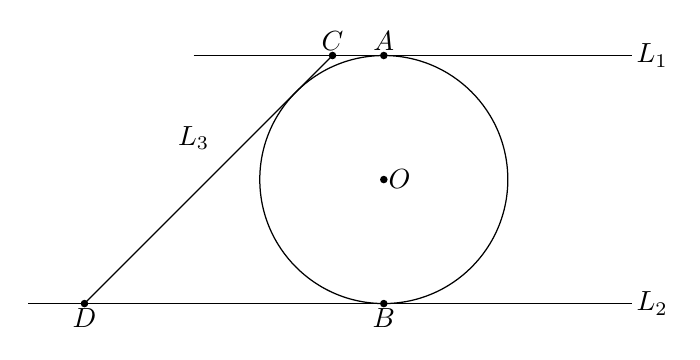
\begin{tikzpicture}[scale=1.05, line width=0.45pt,
  every node/.style={inner sep=1.5pt}]
  \coordinate (O) at (0,0);
  \coordinate (A) at (0,1.5);
  \coordinate (B) at (0,-1.5);
  \coordinate (C) at (-0.62,1.5);
  \coordinate (D) at (-3.62,-1.5);
  \draw (-2.3,1.5) -- (3,1.5);
  \draw (-4.3,-1.5) -- (3,-1.5);
  \draw (O) circle (1.5);
  \draw (C) -- (D);
  \fill (A) circle (1.3pt);
  \fill (B) circle (1.3pt);
  \fill (C) circle (1.3pt);
  \fill (D) circle (1.3pt);
  \fill (O) circle (1.3pt);
  \node[anchor=south] at (A) {$A$};
  \node[anchor=north] at (B) {$B$};
  \node[anchor=south] at (C) {$C$};
  \node[anchor=north] at (D) {$D$};
  \node[anchor=west] at (O) {$O$};
  \node[anchor=west] at (3,1.5) {$L_1$};
  \node[anchor=west] at (3,-1.5) {$L_2$};
  \node at (-2.3,0.5) {$L_3$};
\end{tikzpicture}
